\chapter{Preliminary Evaluation}
\label{chapter:preliminary_evaluation}
To answer the above-mentioned research questions, a preliminary evaluation was conducted. Optimizing and improving our approach with the help of feedback from the participants is the primary goal of this master thesis. Further, we want to learn which status and moods knowledge workers share with their closest team members, what they learn from their team-mates' sharing, and the overall impact on their perception of workplace isolation, which can help us develop both the study and the tool further.

The timeline of the preliminary evaluation is shown in \autoref{fig:study_timeline}. Before the study was officially started with the kick-off meeting with the whole team, each participant was asked to sign and return the consent form (see \autoref{chapter:consent_form}). Additionally, each participant was kindly asked to fill out a questionnaire containing some demographic questions, as well as a 10-item questionnaire about their perception of workplace isolation. During the kick-off meeting, the possibility to ask any questions the participants may have regarding the consent form will be given. The goal of the kick-off meeting was to install AmbientTeams and to show the individual features to the team. Following the kick-off meeting, AmbientTeams is used during at least three workdays. After that, but before the final interview, another questionnaire is sent to the participants.

\begin{figure}[h]
    \centering
    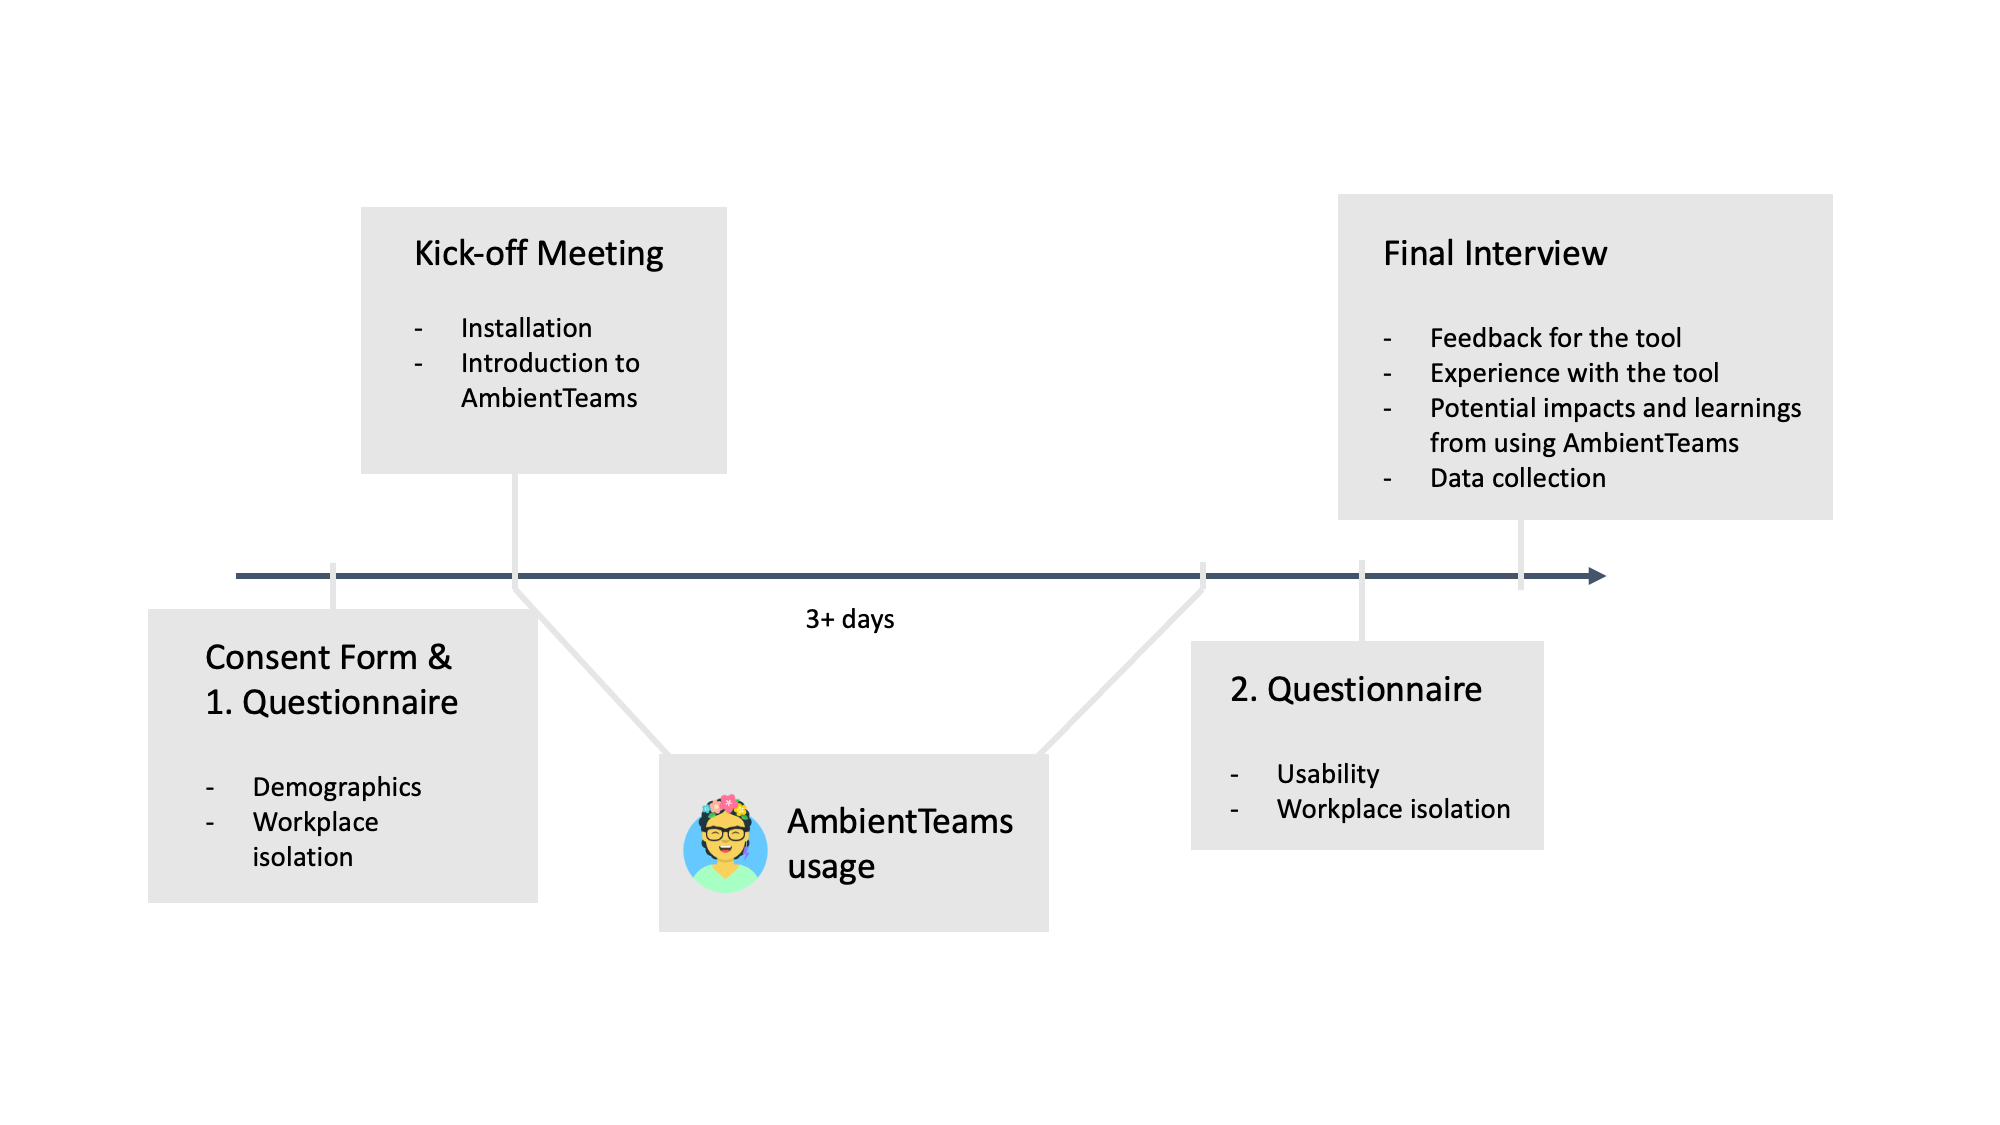
\includegraphics[width=.8\linewidth]{./images/Study_Timeline.png}
    \caption{Study timeline}
    \label{fig:study_timeline}
\end{figure}

In the following sections, we present more details about the study procedure.

\section{Participants Recruitment}
\label{section:recruitment}
As a first step, an interested team had to be recruited. To that end, the researchers' personal network was used. To that purpose, the study description is forwarded to the contacts, and once an interested team has been identified, it is checked whether it fulfills the participation criteria and if the prospective participants are (technically) allowed to install AmbientTeams on their computer. If this is not the case, the company's consent and approval to install AmbientTeams is first obtained. To provide the company with as much information as possible about the study and the confidentiality of the data collected, the consent form and a study description will be given to the company for review. After gaining the company's approval, the individual interested team members are approached by presenting the study, discussing the steps and goals of the study, and emphasizing that participation is entirely voluntary. For the participants to stay anonymous, each participant is assigned a random pseudonym, e.g., P392, which they were asked to provide as answers to the first question in both questionnaires. The requirements for teams participating were:

\begin{enumerate}
    \item At least three team members
    \item Three or more common working days a week
    \item Spending the majority of their workday on the computer
    \item Working remotely as much as possible (ideally completely remote)
    \item Having all the required rights to install AmbientTeams on their work computer
    \item Willingness to use AmbientTeams during at least three full days of work
    \item Using macOS or Microsoft Windows
    \item An active internet connection
\end{enumerate}


\section{Pre-Study Questionnaire}
\label{section:prestudy_questionnaire}
The pre-study questionnaire contains some basic demographic questions, as well as an established workplace isolation questionnaire developed by \textcite{marshall2007workplace}. The demographic questions ask about age, gender, work industry, work experience, and job title. Further, a sense of the team's current communication culture is obtained, whether they are aware of their co-workers' feelings and progress, and the preferred working style (remote vs. onsite) is gathered for each participant. The workplace isolation questionnaire is used as a baseline measurement, and the same questionnaire is also asked at the end of the study, before the final interview, to gain potential first insights into whether our approach can decrease the perception of workplace isolation amongst knowledge workers. The workplace isolation questionnaire contains ten questions and employs a 7-point Likert-Scale, where 1 stands for \enquote{strongly disagree}, and 7 stands for \enquote{strongly agree}. Finally, the participants could optionally write down their expectations for the study. The complete pre-study questionnaire can be found in \autoref{chapter:prestudy_questionnaire}.

\section{Initial Meeting}
\label{section:initial_meeting}
Due to the relatively small number of team members and their flexibility, it was possible to have one kick-off meeting with the entire team. During this meeting, the consent form (see \autoref{chapter:consent_form}) and study instructions (see \autoref{chapter:study_instructions}) were discussed briefly, and opportunities for asking questions were given. Then, we guided the participants through the installation process and explained and demonstrated the functionality of AmbientTeams. Finally, each participant joined the team that we had created before the meeting. Following the kick-off meeting, the study period officially began.

\section{Evaluation Phase}
\label{section:evaluation}
The team voluntarily offered to use AmbientTeams for one workweek as opposed to the three days that were planned initially. During this period, the participants were instructed to continue working as usual. The participants were instructed to contact us should there be an issue or have any other feedback. For very short feedback, AmbientTeams also has a simple feedback-sending feature. During this evaluation phase, application usage data is collected. To that end, \autoref{table:data} shows an overview of all data collected and what research question they are relevant for, together with the location of storage (local vs. server). Local refers to the participants' computers, whereas server refers to the server hosted at the Department of Informatics at the University of Zurich. In other words, the data stored on the server is automatically shared with the researchers. At the same time, only the participants can access the locally stored data unless explicitly shared at the end of the study.

\begin{table}[h]
    \centering
    \begin{tabular}{|p{8cm}|p{1cm}|p{2cm}|}
        \hline
        Data collected                                                                                                                                                     & Storage & Relevance \\
        \hline
        \textbf{User}: email, display name, hashed password, the teams the user belongs to, avatar created on signup                                                       & Server  & -         \\
        \hline

        \textbf{Teams}: name of the team and belonging team members                                                                                                        & Server  & -         \\
        \hline

        \textbf{Status/direct messages}: timestamp, content, team, and user(s) the message belongs to                                                                      & Server  & RQ2, RQ4  \\
        \hline
        \textbf{Availability status}: timestamp, selected availability status, user                                                                                        & Server  & RQ4       \\
        \hline
        \textbf{1:1 calls}: start/end timestamp, call participants                                                                                                         & Server  & RQ4       \\
        \hline
        \textbf{Breakroom}                                                                                                                                                 & Server  & RQ4       \\
        \hline
        \textbf{Nudging}                                                                                                                                                   & Server  & RQ4       \\
        \hline
        \textbf{Random calls}                                                                                                                                              & Server  & RQ4       \\

        \hline
        \textbf{Moods}: timestamp, selected mood, user                                                                                                                     & Server  & RQ4       \\
        \hline
        \textbf{Feedback}: content, user                                                                                                                                   & Server  & -         \\
        \hline
        \textbf{Window actions}:  timestamps of opening, minimizing, closing, or restoring windows that belong to AmbientTeams                                             & Local   & RQ4       \\
        \hline
        \textbf{App running time}:  timestamps of manually starting or quitting AmbientTeams                                                                               & Local   & RQ4       \\
        \hline
        \textbf{Team changes}: timestamps and destination team when switching teams inside AmbientTeams (ambient window)                                                   & Local   & -         \\
        \hline
        \textbf{Active windows}: information about the active windows while ambient teams is running (see https://github.com/sindresorhus/active-win for more information) & Local   & -         \\
        \hline
    \end{tabular}
    \caption{Data collected during the preliminary evluation and its relevance for the RQs}
    \label{table:data}
\end{table}


\section{Post-Study Questionnaire}
\label{section:poststudy_questionnaire}
After the evaluation phase, the participants were asked to fill out another questionnaire, which, similarly to the pre-study questionnaire, takes about 5 minutes to complete. In addition to some control questions about the extent to which the participants worked remotely during the study and how long AmbientTeams was approximately running in the foreground, a usability questionnaire is presented. Usability is measured using the System Usability Score (SUS) introduced by \textcite{brooke1996sus}. As mentioned before, the last block of the post-study questionnaire is the same workplace isolation questionnaire that was answered in the pre-study questionnaire. The complete post-study questionnaire can be found in \autoref{chapter:poststudy_questionnaire}.

Together with the pre-study questionnaire, the goal of the post-study questionnaire is to find insights into a potential impact of AmbientTeams on the perceived workplace isolation, and thus. Also, the SUS will help us better understand and quantify the usability of our approach.

\section{Semi-Structured Final Interview}
\label{section:interview}
Complementing the quantitative data collected during the study, semi-structured final interviews are conducted with each participant individually. The goal of those interviews is to find valuable insights into the usage of AmbientTeams, its strengths, weaknesses and impacts, their sharing behavior. All the interview questions and their relevance for the research questions can be found in \autoref{chapter:interview_guide}. The interviews are designed to take approximately 45 minutes per participant, including the time required to export the local data at the start of the final interview. Because of the potentially confidential information contained in the collected data, participants are free to obfuscate the contents of the active windows file before uploading it to UZH dropfiles\footnote{\url{https://dropfiles.uzh.ch/}}. The interviews are recorded, if the participant allows, and then transcribed. Two researchers (one being the author of this thesis) independently open-coded the transcripts to analyze the interviews.

\section{Participants}
Using our private network of contacts, we were able to find an interested team for the preliminary evaluation. The group initially consisted of six knowledge workers working at a Swiss company operating in the FinTech sector. Unfortunately, one person was eliminated from the study because this person was inactive when using AmbientTeams and could not be reached even after several attempts. The remaining five people consisted of three employees who had been part of the company for about two years, and two had joined their team about three months ago when the study started. While all participants were between 25 and 34 years old, their work experience ranged from 3 (working student) to 13 years (senior accountant). Out of the five participants, three were female, and two male.